%% Springer Nature LaTeX template (sn-jnl) — Discover Artificial Intelligence submission.
%% Compiles with pdflatex (two passes for cross-references/citations).
\documentclass[pdflatex,sn-basic,Numbered]{sn-jnl}

\usepackage{graphicx}
\usepackage{multirow}
\usepackage{amsmath,amssymb,amsfonts}
\usepackage{booktabs}
% The body was being set in Type3 BITMAP fonts (30 of them): with [T1]{fontenc} and no
% scalable T1 Computer Modern installed, pdfTeX falls back to Metafont bitmaps. Type3
% glyphs are rasterised images with no Unicode mapping, so every dash and ligature came
% out of the PDF text layer as its raw encoding slot -- an en dash as 0x15, giving
% ``71.893.7'' for ``71.8--93.7''. Latin Modern is a scalable Type1 T1 font and fixes
% the cause; cmap then emits the ToUnicode CMap.
\usepackage{lmodern}
\usepackage{cmap}% must precede fontenc: emits the ToUnicode CMap for Type1 fonts
\usepackage[T1]{fontenc}
% Without these the PDF text layer carries no Unicode mapping for the dash glyphs, so
% copying a range out of the PDF gives ``71.893.7'' instead of ``71.8--93.7'' -- the
% defect Reviewer 2 reported. \pdfgentounicode makes pdfTeX emit the ToUnicode map.
\input{glyphtounicode}
\pdfgentounicode=1

\raggedbottom

\usepackage{soul}
\usepackage{xcolor}
\definecolor{HLyellow}{rgb}{1,0.94,0.35}
\definecolor{HLink}{rgb}{0.75,0.18,0.04}
\usepackage[normalem]{ulem}
\sethlcolor{HLyellow}
\newcommand{\HLtext}[1]{\texthl{#1}}
\newcommand{\HLcode}[1]{\texthl{#1}}
\newcommand{\HLdel}[1]{\textcolor{HLink}{\sout{#1}}}
\newcommand{\HLtag}[1]{{\color{HLink}\bfseries [#1]~}}
\newcommand{\HLhead}[1]{\textcolor{HLink}{#1}}
\makeatletter
\@ifundefined{pdfstringdefDisableCommands}{}{%
  \pdfstringdefDisableCommands{%
    \renewcommand{\HLhead}[1]{#1}\renewcommand{\HLcode}[1]{#1}%
    \renewcommand{\HLtext}[1]{#1}\renewcommand{\HLdel}[1]{#1}%
    \renewcommand{\HLtag}[1]{}}}
\makeatother
\newcommand{\HLlegend}{%
\par\noindent\fbox{\parbox{0.95\linewidth}{\footnotesize\textbf{Marked copy, revision 1.} Text added since the original submission is \HLtext{highlighted in yellow}. Text removed since the original submission is shown as \HLdel{red struck-through text} at the point where it stood. Table and algorithm bodies are reproduced in final form without internal marks. A float that is new or revised is labelled in its caption, e.g. \HLtag{New in revision}. Page and float numbering match the clean manuscript.}}\par\vspace{6pt}}
\begin{document}

\title[AI foundation model choice and AML false positive variation]{AI foundation model choice and false positive variation in Anti Money Laundering (AML) transaction screening}

\author[1]{\fnm{Samir} \sur{Chincholikar}}\email{samir.chincholikar@gmail.com}

\author*[1]{\fnm{Robin} \sur{Chawla}}\email{robin.chawla.cse14@iitbhu.ac.in}

\affil*[1]{\orgname{Independent Researcher}}

\abstract{Large language models (LLMs) are increasingly considered for anti-money-laundering (AML) transaction screening, but the operational \HLdel{implications of choosing one foundation model over another are poorly quantified. This study investigates} \HLtext{consequences of model choice are poorly quantified. We investigate} how foundation-model selection affects the screening operating point \HLdel{for a fixed task, transaction cases and evaluation procedure. We tested five off-the-shelf foundation models from two providers as zero-shot AML screeners, using a preregistered, fully} \HLtext{when the task, cases and evaluation procedure are held fixed. Five off-the-shelf models from two providers were tested as zero-shot screeners on a preregistered,} reproducible battery of 600 synthetic transaction cases anchored on established laundering typologies, \HLdel{with equal numbers of suspicious cases and legitimate hard negatives designed to resemble common alert patterns.} \HLtext{half suspicious and half hard negatives.} For the same 300 legitimate cases, false-positive rates ranged from \HLdel{0.3\% to 83.0\%---an 82.7 percentage-point spread---and the models disagreed on 85.7\% of legitimate cases. The differences were systematic: false-positive} \HLtext{2.3}\% \HLtext{to 85.7}\%\HLtext{---an 83.3 percentage-point spread (95}\% \HLtext{confidence interval 71.8 to 93.7 points, cluster bootstrap over eight case-template strata)---and the models disagreed on 88.7}\% \HLtext{of legitimate cases. Differences were systematic:} rates decreased monotonically with model tier within each \HLdel{provider family, so that smaller, lower-tier models substantially over-flagged legitimate activity relative to their more capable counterparts. The models therefore occupied quite different points along} \HLtext{of the two provider families studied, so lower-tier models over-flagged legitimate activity. The models occupied different points on} the sensitivity--specificity trade-off, not merely different \HLdel{levels of accuracy. In an illustrative low-prevalence} \HLtext{accuracy levels. In an illustrative} scenario of one million transactions per \HLdel{day, the observed operating points differed by about 200-fold in projected daily alert workload. These findings show that foundation-model choice is} \HLtext{day at 0.1}\% \HLtext{prevalence, projected daily alert workload differed by 36- to 196-fold across the four deployable single-call configurations and by about 35-fold under the preregistered per-case aggregate, with model ordering invariant across prompts, seeds and prevalence. Foundation-model choice is therefore} not merely an AML procurement\HLdel{or implementation}  decision but a core operational risk parameter. Because commercially accessed models may be updated, \HLdel{substituted, repriced or retired by providers, model identity and operating-point stability should be explicitly incorporated into model-risk governance, validation and ongoing monitoring.} \HLtext{substituted or retired by providers, model-tier substitution and alias redirection should be treated as first-class model-risk events, and operating-point stability monitored through a standing probe.}}

\keywords{anti-money laundering, foundation models, false positives, model risk, large language models, transaction monitoring}

\maketitle
\HLlegend


\section{Introduction}\label{sec:intro}

Money laundering is estimated to account for 2--5\% of global gross domestic product each year, and financial institutions operate under AML frameworks requiring ongoing transaction monitoring and the reporting of suspicious activity \cite{fatf-recs,unodc}. In practice, transaction-monitoring systems generate large numbers of alerts for compliance analysts to review. Traditional rule-based systems have been widely criticised for very high false-positive rates, often reported to exceed 90\% of all alerts \cite{jensen}. These false alarms generate substantial operating costs, consume investigative resources, and can lead to unwarranted customer friction and de-risking. Minimising the false-positive burden, while retaining sufficient sensitivity to genuinely suspicious activity, therefore remains one of the central technical and operational challenges in anti-money-laundering (AML) monitoring \cite{alhashedi,smote,goecks,imbalance}.

Machine-learning methods have been introduced into AML and related financial-crime applications largely to improve this trade-off. Existing research in this domain includes supervised classifiers, ensemble methods, deep-learning architectures, resampling techniques for severe class imbalance, federated learning, and explainability methods such as SHAP and LIME \cite{alhashedi,disc-alshatri,disc-bekkaye,goecks,imbalance,shap,disc-najem,lime,disc-yang,amlsim}. Large language models (LLMs) and other general-purpose foundation \HLdel{models---trained} \HLtext{models} \cite{fewshot,foundation}\HLtext{---trained} on broad data and adapted to many tasks through natural-language \HLtext{instructions---have} recently gained attention for their ability to interpret heterogeneous information without the need for task-specific retraining. In principle, an LLM-based screener can reason about known laundering typologies while analysing transaction histories, account attributes, counterparties, jurisdictions and behavioural patterns. Such flexibility makes foundation models attractive to institutions seeking to augment or modernise legacy monitoring systems.

However, most existing evaluation is framed primarily as a model-capability problem: how well can a particular model identify suspicious activity? Most studies evaluate a single model, or compare a few models to identify the one with the highest accuracy, recall, F1-score or related performance metric \cite{disc-alshatri,disc-bekkaye,disc-najem,disc-yang}, mirroring the model-centric emphasis of general LLM evaluation and of the broader debate over the reliability of large models \cite{helm,parrots}. This framing implicitly treats the identity of the underlying foundation model as an implementation detail. Once the model is selected, governance usually proceeds to monitoring for performance degradation due to data drift, concept drift or a change in the operating environment.

This assumption holds for a traditional model in which the institution still controls the weights, the training process and the deployed artefact. It is less applicable to foundation models accessed through commercial application programming interfaces (APIs). In such deployments, the institution may not control the model weights, the lifecycle of a particular model version, or the provider's decisions to update, replace, re-price, route or retire models. Two deployments with identical screening logic and identical transaction data can behave differently solely because they use different foundation models. Moreover, a provider-side change to the model can alter system behaviour without any retraining event or data-distribution shift that a traditional drift-monitoring process would necessarily detect.

This issue is particularly important in AML because the relevant operational quantity is not aggregate accuracy alone. The effective operating point of a screening system is determined by the trade-off between false positives and missed suspicious cases. A model that maximises sensitivity by flagging nearly all cases may appear successful at detecting suspicious activity, yet produce an operationally unsustainable alert queue. Conversely, a very conservative model may dramatically reduce false positives while allowing a higher proportion of suspicious activity to pass. Foundation-model selection may therefore determine not only which model is ``better'' but also where the deployed system lies on the sensitivity--specificity trade-off.

Much of the wider financial-crime literature has focused on reducing false positives through class-imbalance correction, cost-sensitive learning, model optimisation, ensemble methods and better feature representations \cite{alhashedi,smote,goecks,imbalance}. Other work has investigated post-hoc explainability for the individual auditability of alerts \cite{shap,lime} and predictive or graph-based AML monitoring \cite{jullum,pourhabibi}. More recent continual-learning research explicitly addresses evolving laundering patterns and model adaptation over time \cite{deprez}. These techniques are useful, but they generally assume that the monitored model is a stable artefact. They do not directly account for the fact that switching from one commercially available foundation model to another could cause a large change in false-positive and miss rates even when the task and input transactions remain unchanged.

Relatedly, the literature on algorithmic monoculture raises concerns that heavy dependence on a small set of shared foundation models may lead institutions to make similar decisions and to suffer correlated errors \cite{homogenization,leviathan,monoculture}. This leaves two competing possibilities for AML screening. Shared foundation models may converge, producing common blind spots on the same suspicious cases, or they may diverge greatly, returning different results for identical transactions depending on the model used. We are not aware of \HLdel{any direct measurement of this cross-model divergence at scale under a controlled AML screening design.} \HLtext{a preregistered measurement that translates this divergence into screening operating points and alert burden.}

The study therefore asks a different question from traditional model-comparison research: \emph{how does the choice of foundation model change the AML screening operating point when the screening task and transaction cases are held fixed?}

To this end, we evaluate five commercially available foundation models from two providers as zero-shot AML screeners on a common, preregistered battery of 600 synthetic transaction cases based on recognised Financial Action Task Force (FATF) laundering typologies and established synthetic-AML data structures \cite{samld,weber2018}. The battery includes 300 suspicious cases drawn from eight laundering typologies and 300 legitimate hard-negative cases that resemble typical alert-generating patterns. Synthetic cases with complete ground-truth labels, controlled variation, identical inputs across models and full reproducibility are used deliberately. The goal is thus not to estimate absolute production-bank false-positive or miss rates, but to measure the change in operating point between models for fixed underlying cases.

Each model is evaluated on all cases under two formulations of the supervisory prompt and two random seeds, allowing us to separate model-level divergence from prompt-level sensitivity. We measure false-positive rates, miss rates, cross-model disagreement, typology-specific behaviour and prompt \HLdel{sensitivity;} \HLtext{sensitivity. We} compare the models with deterministic rules and supervised machine-learning \HLdel{baselines;} \HLtext{baselines,} and translate the measured operating points into an illustrative low-prevalence alert-volume scenario. As a preregistered secondary analysis, we also test whether the models show correlated misses as predicted by the algorithmic-monoculture hypothesis.

The study makes three main contributions:

\begin{enumerate}
\item \HLdel{\emph{Controlled measurement of foundation-model selection risk.} To the best of our knowledge, this is the first study to control foundation-model identity as the experimental variable in AML transaction screening while fixing the task and transaction cases.} \emph{A foundation-model-swap interpretation of model governance.} \HLtext{We treat model-tier substitution and provider-managed} \texttt{-latest} \HLtext{alias redirection as first-class model-risk events, and propose a standing operating-point probe as a monitoring control, so that the specific model version and its operating point become part of model inventories, validation procedures and ongoing monitoring} (Section~\ref{sec:probe}\HLtext{).}
\item \emph{Domain-specific controlled measurement.} \HLtext{That different language models disagree on identical inputs, and that model-induced variance can exceed prompt-induced variance, is established in the broader model-evaluation literature} \cite{helm,promptsens}\HLtext{. Our contribution is not the phenomenon but its first preregistered, governance-framed controlled measurement in AML transaction screening: foundation-model identity is the experimental variable, while the task, the transaction cases, the prompts and the evaluation procedure are held fixed.}
\item \emph{Operational impact quantification.} We quantify differences in false-positive and miss rates via paired statistical tests and \HLtext{cluster-robust} uncertainty estimates, compare the resulting operating points to non-LLM baselines, and translate the differences into expected alert workload under an illustrative low-prevalence operating scenario.
\end{enumerate}

In sum, the analysis moves the question from whether LLMs can perform AML screening to the governance-relevant question of whether different foundation models perform the same screening task well enough to be treated as interchangeable components.

\section{Methods}\label{sec:methods}

\subsection{Study design and case battery}

The study was designed to isolate the effect of foundation-model identity on AML screening decisions. All evaluated models were therefore given the same transaction cases under the same screening task, while the underlying foundation model was varied. The goal was not to estimate production-bank false-positive or miss rates, but to quantify how much the screening operating point changes when the model is changed and the transaction evidence is held constant.

We created a deterministic offline battery of 600 synthetic cases with seed \texttt{20260715}. The cases were derived from recognised FATF laundering typologies and from the structure of established synthetic-AML datasets, including SAML-D and the IBM AMLSim lineage \cite{samld,weber2018}. Each case was a small transaction sub-network, serialised as a plain-text ledger with account-level attributes (including know-your-customer and jurisdiction information) and transaction-level attributes (amount, date, direction and payment channel).

The battery was balanced by design. Three hundred cases represented suspicious activity, spread across eight laundering typologies: structuring, layering, trade-based laundering, mule networks, shell layering, funnel accounts, rapid pass-through activity, and cash-intensive fronts. The other 300 cases were legitimate hard negatives. These benign cases included patterns such as payroll processing, treasury sweeps, documented trade-finance activity and marketplace payouts that might appear superficially similar to traditional AML red flags. Hard negatives were included deliberately to prevent a model from performing well simply by flagging every case as suspicious.

Several design features were incorporated to mitigate trivial label leakage. The cases were raw transaction records rather than natural-language \HLdel{summaries; suspicious} \HLtext{summaries. Suspicious} cases used irregular sub-threshold amounts rather than mechanically uniform \HLdel{ones; laundering} \HLtext{ones. Laundering} signals were interleaved with legitimate background \HLdel{transactions;} \HLtext{transactions,} and relevant activity was temporally dispersed. We retained the generator, the case battery it produced, and its SHA-256 hash as part of the reproducibility package. The reproduction workflow regenerates the battery from the fixed seed and checks the resulting file against the stored hash.

The use of synthetic data was an intentional, controlled design choice. Real-world AML transaction data with complete ground-truth labels is extremely limited, and confirmed real-world labels are inherently incomplete because undetected laundering cannot be presented as a known positive case. The synthetic battery allows full labelling, submission of the same cases to all evaluated models, control over the presence of typology-specific signals, and complete reproducibility. The measured absolute error rates are therefore properties of this controlled evaluation battery, not estimates of production-bank performance. The primary estimand is the difference between models in screening behaviour on identical cases.

\HLtext{Case labels are correct by construction of the generator: a case is suspicious because it was instantiated from one of the eight FATF-anchored typology templates, and legitimate because it was instantiated from a hard-negative template. No independent anti-money-laundering expert reviewed or adjudicated any part of the battery, and no inter-rater reliability check was performed. The false-positive and miss rates reported here are therefore measured against template-defined ground truth rather than against expert judgement, a limitation discussed in} Section~\ref{sec:limits}\HLtext{. Each legitimate case is assigned to the stratum of the benign pattern its hard-negative template instantiates. The legitimate and suspicious sides therefore carry eight strata each, drawn from two disjoint sets of templates: eight benign patterns and eight laundering typologies. The case-template strata are used as clustering units for cluster-bootstrap confidence intervals and cluster-level permutation tests. Wilson score intervals for individual model proportions remain case-level intervals.}

\subsection{\HLhead{Foundation models and screening procedure}}\label{sec:design}

We evaluated five commercial foundation models from two providers:

\begin{itemize}
\item OpenAI GPT-4o-mini (\texttt{gpt-4o-mini-2024-07-18}\HLtext{)}
\item \HLtext{OpenAI GPT-4.1-mini (}\texttt{gpt-4.1-mini-2025-04-14}\HLtext{)}
\item \HLtext{OpenAI GPT-4o (}\texttt{gpt-4o-2024-11-20}\HLtext{)}
\item \HLtext{Google Gemini Flash}
\item Google Gemini Flash-Lite.
\end{itemize}

The OpenAI models were accessed through dated snapshot identifiers, which lock requests to specific model versions \cite{openai-models}. The Google models were accessed through the provider-managed aliases \texttt{gemini-flash-latest} and \texttt{gemini-flash-lite-latest}\HLtext{.} Google documents these \texttt{-latest} identifiers as aliases that can be hot-swapped as newer releases become available \cite{google-models}. \HLdel{The exact model} \HLtext{Only the alias strings were captured: the concrete model version} served behind each Google alias at the collection date (July 2026) \HLdel{is} \HLtext{was not} recorded in the archived per-call \HLdel{response metadata (see Data availability), rather than inferred from the alias.} \HLtext{metadata and cannot now be recovered. This is itself an instance of the governance problem examined here, and it is stated again among the limitations.} Unlike the OpenAI identifiers, the Google aliases did not expose an immutable, dated snapshot identifier. This distinction is relevant to the governance question considered here, because an alias can alter the model underlying an application without any corresponding change in the institution's own code.

All models were evaluated as zero-shot screeners. We did not fine-tune any model on the case battery, nor perform any model-specific prompt optimisation. Every model was given the same representation of the case and asked to classify the activity as suspicious or not suspicious.

To assess whether the wording of the instructions had a meaningful \HLdel{effect---a} \HLtext{effect} \cite{promptsens}\HLtext{---a} known source of variation in LLM \HLtext{behaviour---each} case was tested with two versions of the supervisory prompt: a short instruction for a compliance officer, and a more elaborate instruction aware of the FATF typologies. Each prompt setting was run twice with different random seeds. The complete design therefore comprised \HLdel{$5 \text{ models} \times 2 \text{ prompt formulations} \times 2 \text{ seeds} \times 600 \text{ cases} = 12{,}000$ screening calls.} \HLtext{five models, two prompt formulations, two seeds and 600 cases, giving} 12{,}000 \HLtext{screening calls by design. The frozen corpus holds} 12{,}120 \HLtext{calls: 111 GPT-4o-mini cases carry a fifth retried call and one GPT-4.1-mini case carries three valid calls after an application-programming-interface error. The 111 retries were made because the GPT-4o-mini terse-prompt seed-0 pass was re-issued after OpenAI rate limiting interrupted it, so cases that had already returned were called a second time. The remaining 9 calls are ERROR rows recording the rate-limit failures themselves, which are excluded from the vote. For these cases the single-call analysis uses one of the two terse seed-0 calls and both enter the per-case vote, so the cell is decided on five valid calls rather than four. The two calls returned the same decision in all 111 cases, so the single-call analysis is unaffected by the choice. In the vote the extra call changes one legitimate GPT-4o-mini decision, which would otherwise be an even split resolved toward} \texttt{flag}\HLtext{, lowering that model's false-positive rate by 0.3 percentage points. Duplicate calls are retained in the archive for auditability. Restricting the vote to the four designed prompt--seed cells gives GPT-4o-mini a false-positive rate of 86.0}\% \HLtext{and a cross-model spread of 83.7 percentage points. We report aggregation over all valid calls as primary because D4 specifies the ``modal replicate decision across seeds} $\times$ \HLtext{prompt variants'' with ``ERROR replicates excluded from the vote'', defining the vote over valid replicate calls rather than over a fixed count of four, and the four-cell aggregation as a sensitivity analysis. Both the designed and the realized counts are reported because the retries were made during capture and are preserved in the archive.}

The models were run at temperature 0 and returned a constrained JSON object with the suspicious/not-suspicious decision. Calls that failed or produced unparsable output were logged as errors rather than silently coerced into a valid \HLdel{class; the} \HLtext{class. The} overall call-level error rate was 0.08\%. For the primary per-case analysis, valid replicate decisions were aggregated at the case level according to the prespecified voting procedure, and failed calls were excluded from the aggregation. The exact voting rule---including the treatment of ties and failed calls---is given in Appendix~A.

\HLtext{The evaluated set is the surviving part of a larger preregistered grid. The confirmatory design specified a third provider family, xAI Grok-4.5, alongside the OpenAI and Google models. Two logged decisions reduced it: D17 dropped} \texttt{gemini-pro} \HLtext{for thinking-mode incompatibility and cost, and D19 dropped} \texttt{xai-grok} \HLtext{because the xAI account was out of credits before the full run. The final grid of five models from two providers is therefore the result of documented attrition rather than a two-provider design, and, because tier is defined only within providers, a provider main effect cannot be separated from the tier effect. Anthropic Claude appears in the generative-artificial-intelligence declaration solely as a coding assistant and was never an evaluated system.}

Because foundation models and commercial interfaces can be updated or retired by providers, model identifiers and access conditions were recorded at the time of data collection. During the study, one provider deprecated a selected model snapshot, which had to be substituted during data collection. This event is recorded because it directly illustrates the model-lifecycle risk studied in this paper.

\subsection{\HLhead{Per-case aggregation rule and a deviation from it}}\label{sec:agg}

\HLtext{Each (model, case) pair carries four valid calls by design, two prompt formulations crossed with two seeds. Preregistered} decision~D4 \HLtext{reduces them to one decision per case by the modal replicate decision, with ties broken toward} \texttt{flag}\HLtext{. The rule is stated in the decisions log and repeated in both preregistration documents, and it makes no reference to the ground-truth label of the case. That label-independent rule is the primary rule throughout this paper.}

\HLtext{The analysis submitted for review departed from it. On legitimate cases it required a strict majority, so a 2--2 split was not counted as a false positive, while on suspicious cases it followed D4 and counted a 2--2 split as caught. The tie direction therefore depended on the known case label, and in both branches it favoured the model. The departure was not disclosed at submission and is corrected here. Its likely origin is the change of estimand: D4 is justified in the decisions log on the ground that breaking ties toward} \texttt{flag} \HLtext{keeps the} \emph{miss} \HLtext{estimate conservative, which held while the endpoint was misses. Once the endpoint became false positives, conservatism appears to have been reapplied separately to each endpoint.}

\HLtext{Restoring D4 raises every false-positive rate---from 0.3, 1.0, 23.7, 24.7 and 83.0}\% \HLtext{to 2.3, 7.7, 37.0, 44.0 and 85.7}\%\HLtext{---and leaves every miss rate unchanged, because the suspicious branch already followed D4. The cross-model spread, which carries the paper's main claim, moves from 82.7 to 83.3 percentage points. Ties are not uniformly distributed: on legitimate cases they number 6, 20, 40, 58 and 8 for Gemini Flash, GPT-4o, GPT-4.1-mini, Gemini Flash-Lite and GPT-4o-mini respectively, and on suspicious cases 19, 15, 10, 4 and 0. They concentrate where a model sits near its own decision boundary, so the deviation compressed the middle of the distribution rather than its extremes.}

\HLtext{Because the choice of rule is consequential, the results are reported under four further label-independent policies and under each deployable single-call configuration} (Table~\ref{tab:agg}\HLtext{). Across all nine analyses the spread lies between 77.7 and 85.3 percentage points and no pair of models reverses order.}

\HLtext{Two further points follow. First, the four-call aggregate is an evaluation construct rather than an operationally validated multi-call screening configuration. A multi-call implementation is possible but would require separate assessment of cost, latency and screening workflow. The deployable quantity is a single call, and those configurations are reported alongside the aggregate. Second, a label-independent rule that resolves ties by strict majority on both labels reproduces the submitted false-positive rates exactly but raises miss rates from 12.0, 3.3, 3.7, 0.7 and 0.0}\% \HLtext{to 18.3, 8.3, 7.0, 2.0 and 0.0}\%\HLtext{. The submitted false-positive rates are therefore attainable without the label, at a cost on the miss axis.}

\subsection{Endpoints and statistical analysis}

The main outcome was the false-positive rate for each model on the 300 legitimate cases, where a false positive is a legitimate case classified as suspicious. The main cross-model estimand was the spread in false-positive rates, defined as the maximum minus the minimum false-positive rate across the five models. Secondary outcomes were the rate of missed suspicious cases, cross-model disagreement on valid cases, miss rates by typology, sensitivity to prompt wording, and chance-corrected agreement between models.

Because all five models decided on the same set of transaction cases, their decisions were treated as paired binary observations rather than independent samples. Using Cochran's $Q$ test for related binary samples \cite{cochran}, we tested the overall null hypothesis of equal false-positive rates across the five models ($k=5$ models, $n=300$ legitimate cases, $k-1=4$ degrees of freedom). Where global testing identified model-level heterogeneity, pairwise comparisons used the exact McNemar test on the discordant classifications in each paired model comparison \cite{mcnemar}. Tests were two-tailed with an initial significance level of $\alpha=0.05$. To control the family-wise error rate, a Bonferroni correction was applied across the ten pairwise comparisons among the five models.

\HLtext{Cochran's} $Q$ \HLtext{and the exact McNemar test both treat the 300 legitimate cases as exchangeable units. Because the cases are generated from a shared set of case templates, that assumption is not satisfied exactly. The primary test is therefore accompanied by a cluster-level permutation procedure in which a single permutation of model labels is applied to all cases within each of the eight case-template strata, and the adjacent-tier contrasts are reported with cluster-robust bootstrap intervals over the same strata. With eight clusters, these intervals are approximate. Case-level} $P$\HLtext{-values are retained for comparability with the preregistered analysis plan, and the cluster-robust results are the ones relied upon. The Cochran's} $Q$ \HLtext{statistics reported at submission omitted the factor} $k$ \HLtext{from the numerator and were understated fivefold. All} $Q$ \HLtext{values reported here are corrected and were cross-checked against an independent implementation.}

Proportions such as false-positive and miss rates are reported with 95\% Wilson score confidence intervals \cite{wilson}. For quantities whose uncertainty was composition-dependent across \HLdel{typology strata (cross-model spread, disagreement metrics and typology-level rates),} \HLtext{case-template strata (cross-model spread and disagreement metrics),} additional 95\% percentile bootstrap confidence intervals were constructed via cluster resampling over the eight \HLdel{typology} \HLtext{case-template} strata \cite{bootstrap}, using 2{,}000 bootstrap resamples and seed \texttt{4242}. Terminology is conservative throughout: ``significant'' is used only for comparisons accompanied by a formal $P$-value, and descriptive differences without a formal hypothesis test are characterised as large, substantial or small as appropriate.

Agreement between models was additionally investigated using chance-corrected \HLdel{statistics---Cohen's} \HLtext{statistics} \cite{gwet}\HLtext{---Cohen's} $\kappa$, Scott's $\pi$ and Gwet's \HLtext{AC1---particularly} in the preregistered secondary analysis of whether the models exhibited correlated misses consistent with an algorithmic-monoculture hypothesis. For the within-provider comparison, ``model tier'' \HLdel{follows each provider's contemporaneous capability/product and} \HLtext{is defined operationally as the provider's published} price positioning at the time of data \HLdel{collection---the per-model product identifiers and list prices are recorded in the archived model registry (\texttt{data/configs/models.yaml})---and} \HLtext{collection, with the tier ordering following the price ordering inside each provider family. For the OpenAI models these are the published list prices per million input and output tokens:} \$\HLtext{2.50 and} \$\HLtext{10.00 for GPT-4o,} \$\HLtext{0.40 and} \$\HLtext{1.60 for GPT-4.1-mini, and} \$\HLtext{0.15 and} \$\HLtext{0.60 for GPT-4o-mini} \cite{openai-pricing}\HLtext{. For the Google models the list prices current in July 2026 cannot be substantiated retrospectively, because the models were reached through} \texttt{-latest} \HLtext{aliases whose resolved versions were not captured and which the provider's current pricing page no longer lists. The price fields for those two entries in the archived registry (}\texttt{data/configs/models.yaml}\HLtext{) are conservative budgeting placeholders, not list prices. The tier ordering is therefore corroborated for all five models by the measured cost per call recorded in the archived spend ledger---}\$\HLtext{0.002108 for GPT-4o,} \$\HLtext{0.000536 for Gemini Flash,} \$\HLtext{0.000342 for GPT-4.1-mini,} \$\HLtext{0.000148 for Gemini Flash-Lite and} \$\HLtext{0.000125 for GPT-4o-mini---which is reproducible from the deposit. Measured cost per call is reported as an expenditure measure and may also reflect differences in token usage. It is not interpreted as a direct measure of model capability or size. Tier} is used only within provider families, not as a universal cross-provider capability scale.

\subsection{Non-LLM baselines}

To place the foundation-model operating points in context, we benchmarked two non-LLM reference systems on the same 600-case battery. The first was a deterministic rules-based baseline encoding common FATF-style red-flag heuristics, including sub-threshold structuring, mule-account fan-in, shell-entity transfers, high-risk-jurisdiction wires and rapid pass-through activity. The second was a supervised machine-learning baseline based on engineered graph and transaction features, including counts of cash transactions, sub-threshold transfers, fan-in behaviour, shell-entity involvement, high-risk jurisdictions and temporal-span \HLdel{features; logistic-regression} \HLtext{features. Logistic-regression} and gradient-boosting classifiers were evaluated using five-fold stratified out-of-fold prediction.

The supervised baseline performed well because the synthetic battery was built on familiar laundering structures, so the engineered features were expected to correlate strongly with the data-generating process. Its performance is therefore viewed as an optimistic reference ceiling on this controlled battery, not as an estimate of supervised AML performance in production environments.

\subsection{Operational load projection}

Classification performance on a balanced experimental battery reveals little about the operational workload of AML screening, where suspicious activity is rare in real deployments. Even a model that performs well on aggregate metrics may generate alert queues dominated by false positives. To illustrate the operational implication of the measured operating points, each model was projected onto a hypothetical institution processing $N = 1{,}000{,}000$ transactions per day at a suspicious-activity prevalence of $p = 0.001$. This is a hypothetical low-prevalence scenario and should not be taken as an empirical estimate of prevalence at any financial institution.

For each model, the expected number of alerts per day was computed as
\[
\text{Alerts} = \mathrm{FP}\cdot N(1-p) + (1-\mathrm{Miss})\cdot Np,
\]
where $\mathrm{FP}$ is the measured false-positive rate and $\mathrm{Miss}$ is the measured miss rate. The expected number of false alerts was
\[
\text{False alerts} = \mathrm{FP}\cdot N(1-p),
\]
and the expected alert precision was the expected number of true suspicious alerts divided by the total expected alerts. The objective of this scenario analysis was not to predict the alert volume of any particular institution, but to express the experimentally observed operating-point differences in terms of analyst workload and alert quality.

\subsection{Software, preregistration and reproducibility}

The analysis was performed in Python 3.12 with NumPy 2.2.6, scikit-learn 1.7.2 \cite{sklearn}, SciPy 1.18.0 and Matplotlib \HLdel{3.10; the} \HLtext{3.10. The} OpenAI and Google Python software development kits were used in data collection. The experimental design and main analyses were preregistered prior to data collection. The reproducibility package includes the case generator, the frozen battery of 600 cases, the full corpus of model responses, configuration information, statistical-analysis code, relevant hashes, and preregistration materials. The analysis pipeline is deterministic and reproduces the reported results from the frozen data.

The study distinguishes two types of reproducibility. The analysis is fully reproducible from the archived response corpus, whereas re-querying commercial foundation models at a later date may not reproduce the original responses, because providers can update, replace or retire the underlying models. This distinction is itself pertinent to the model-governance problem studied here.

\section{Results}\label{sec:results}

\subsection{Foundation models show large differences in false-positive rates on identical legitimate cases}\label{sec:fpspread}

The five foundation models screened the complete battery of 600 cases under the same experimental conditions. For the main analysis, model decisions were pooled across the two prompt formulations and two random seeds at the case level. A false positive was a legitimate case classified as suspicious, and a miss was a suspicious case classified as legitimate.

The false-positive rate on the 300 legitimate cases ranged from \HLdel{0.3\% (1} \HLtext{2.3}\% \HLtext{(7} of 300 cases) for Gemini Flash to \HLdel{83.0\% (249} \HLtext{85.7}\% \HLtext{(257} of 300 cases) for GPT-4o-mini. The resulting cross-model spread was \HLdel{82.7} \HLtext{83.3} percentage points (95\% confidence interval [CI] \HLtext{71.8 to 93.7, cluster bootstrap over the eight case-template strata)} (Fig.~\ref{fig:fp}\HLtext{,} Table~\ref{tab:ops}\HLtext{). Under the preregistered aggregation rule, the five models differed in false-positive rate (Cochran's} $Q = 585.0$\HLtext{, 4 df, case-level} $P \approx 2.7\times10^{-125}$\HLtext{). Because cases share generating templates, we also tested the global null using a cluster-level permutation procedure that applies a single permutation of model labels to all cases within each of the eight case-template strata. None of the 2,000 permuted statistics reached the observed value (Monte Carlo} $P \approx 0.0005$\HLtext{, using the plus-one correction). We rely on the cluster-level inference for the principal significance claim.} Pairwise exact McNemar tests (Bonferroni-corrected across the ten possible model comparisons) compared every model pair on the same legitimate cases. \HLdel{Grouping the models by observed false-positive rate into a low pair (Gemini Flash, GPT-4o), an intermediate pair (GPT-4.1-mini, Gemini Flash-Lite), and GPT-4o-mini, all between-group} \HLtext{Nine of the ten} comparisons were statistically significant after \HLdel{correction ($P < 10^{-18}$), whereas the two within-group comparisons were not statistically significant ($P = 1.0$)} \HLtext{correction, the weakest being Gemini Flash versus GPT-4o (}$P = 4.0\times10^{-3}$\HLtext{). The single exception was GPT-4.1-mini versus Gemini Flash-Lite (}$P = 0.76$\HLtext{), two models that occupy the same region of the operating-point space} (Table~\ref{tab:mcnemar}).

The difference was not limited to aggregate rates. The five models did not screen unanimously on \HLdel{85.7} \HLtext{88.7}\% of the legitimate cases (95\% CI \HLdel{75.1--95.4).} \HLtext{82.2--95.0).} For the large majority of hard-negative cases, therefore, whether the case was escalated depended on which foundation model screened the transaction. These results establish that foundation-model identity alone can generate substantial variation in false-positive behaviour when the transaction evidence and screening task are held constant.

\subsection{False-positive rates decrease with model tier within both evaluated provider families}\label{sec:tier}

Consistent within-provider patterns of cross-model variation were observed (Fig.~\ref{fig:ops}\HLtext{,} Table~\ref{tab:ops}). Across the three OpenAI models, the false-positive rate fell from \HLdel{83.0\% for GPT-4o-mini, to 23.7\% for GPT-4.1-mini, to 1.0} \HLtext{85.7}\% \HLtext{for GPT-4o-mini, to 37.0}\% \HLtext{for GPT-4.1-mini, to 7.7}\% for GPT-4o. Across the two Google models, it fell from \HLdel{24.7\% for Gemini Flash-Lite to 0.3} \HLtext{44.0}\% \HLtext{for Gemini Flash-Lite to 2.3}\% for Gemini Flash. In both provider families, the smaller, lower-tier model generated more false positives.

\HLtext{Because the design is fully paired, the ordering was tested by comparing adjacent tiers on the same legitimate cases rather than by a trend test across tiers, which would treat the same 300 cases as independent groups and overstate the evidence. All three adjacent-tier comparisons ran in the predicted direction and remained significant after Bonferroni correction across the three tests: GPT-4o to GPT-4.1-mini (discordant counts 2 and 90, difference 29.3 points, cluster-robust 95}\% \HLtext{CI 12.6 to 51.2), GPT-4.1-mini to GPT-4o-mini (3 and 149, 48.7 points, CI 25.8 to 72.5), and Gemini Flash to Gemini Flash-Lite (0 and 125, 41.7 points, CI 19.7 to 65.2). Each interval excludes zero.} This monotonic pattern should be understood only within the \HLdel{evaluated model} \HLtext{two evaluated provider} families and does not imply a general cross-provider relationship between model size, price or capability and false-positive behaviour.

Reduced false-positive rates were also associated with reduced sensitivity. In the most aggressive screening regime, GPT-4o-mini flagged virtually all suspicious cases but generated false positives on \HLdel{83.0} \HLtext{85.7}\% of legitimate cases. Gemini Flash, by contrast, had the lowest false-positive rate \HLdel{(0.3} \HLtext{(2.3}\%) but missed 12.0\% of suspicious cases. The two intermediate models and GPT-4o lay between these extremes. Plotting sensitivity against false-positive rate therefore shows that the models differed not only in overall predictive quality but occupied materially different screening operating points (Fig.~\ref{fig:ops}): some preferred aggressive escalation, accepting many false alarms, while others suppressed false positives at the cost of a higher miss rate.

The dispersion was especially large among the lower-tier models. Although both are lower-cost models from their providers, GPT-4o-mini and Gemini Flash-Lite differed by about \HLdel{58} \HLtext{42} percentage points in false-positive rate. In contrast, the two higher-tier models, GPT-4o and Gemini Flash, \HLdel{converged near zero false positives, at 1.0\% and 0.3} \HLtext{remained an order of magnitude lower than the most permissive model, at 7.7}\% \HLtext{and 2.3}\% respectively.

\subsection{The operating point translates into a large difference in alert workload}\label{sec:volume}

A balanced experimental battery is useful for comparing discrimination between suspicious and legitimate cases, but AML systems operate in a regime where suspicious activity is rare. Even small differences in false-positive rate can therefore produce large differences in analyst workload in a low-prevalence setting. To demonstrate this effect, the measured operating points were projected onto a scenario of 1,000,000 transactions per day at an assumed suspicious-activity prevalence of 0.1\%. This scenario is illustrative and is not intended as an estimate of prevalence for any particular institution.

Under these assumptions, the expected daily alert volume ranged from roughly \HLdel{4,200} \HLtext{24,000} alerts for Gemini Flash to approximately \HLtext{857,000 alerts for GPT-4o-mini} (Fig.~\ref{fig:vol}\HLtext{,} Table~\ref{tab:vol})---a difference in daily alert workload of about \HLdel{197-fold} \HLtext{35-fold} on the same underlying transaction population. The contents of those alert queues also differed sharply. At the Gemini Flash operating point, the estimated precision was about \HLdel{20.9} \HLtext{3.6}\%, versus about 0.12\% at the GPT-4o-mini operating \HLdel{point; at} \HLtext{point. At} the latter, about 999 of every 1,000 alerts would be expected to be false under the stated prevalence assumption.

\HLtext{The magnitude of this ratio depends on how the replicate calls are reduced to one decision per case, whereas the ordering of the models does not. Under the four deployable single-call configurations} (Section~\ref{sec:agg}\HLtext{) the ratio is 36-fold and 36-fold for the two FATF-prompt configurations and 194-fold and 196-fold for the two terse-prompt configurations, so the defensible range across configurations an institution could actually deploy is 36- to 196-fold. The ordering of the five models by alert volume is identical in every configuration. The magnitude is also prevalence-dependent: sweeping prevalence from 0.01}\% \HLtext{to 1}\% \HLtext{moves the ratio from about 37-fold to about 27-fold while leaving the ordering unchanged} (Fig.~\ref{fig:sweep}\HLtext{), because true positives occupy a growing share of the queue for the low-false-positive models as prevalence rises. Precision moves over the same range from 0.4}\% \HLtext{to 27.6}\% \HLtext{for Gemini Flash and from 0.01}\% \HLtext{to 1.2}\% \HLtext{for GPT-4o-mini.} The operational effect of model selection is thus far greater than aggregate classification metrics alone would imply: a change in foundation model can alter not only detection behaviour but also the number and quality of cases presented to human investigators.

\subsection{Comparison with non-LLM baselines}\label{sec:baselines}

The two non-LLM baselines were evaluated on the same 600 cases to provide a common reference frame. The deterministic rules-based baseline produced a 12.0\% false-positive rate and an 11.3\% miss rate. The supervised classifiers trained on engineered transaction and graph features performed substantially better on the synthetic battery, with the gradient-boosting model achieving near-zero false-positive and miss rates under out-of-fold evaluation.

The strong supervised performance is consistent with the construction of the controlled battery: the cases contain explicit structural manifestations of the laundering typologies, and the engineered features were designed to capture those structures. The supervised result should therefore be regarded as an optimistic reference ceiling for this synthetic evaluation, not an estimate of production AML performance. Against the rules baseline, the foundation models were widely dispersed: GPT-4o-mini had about seven times the false-positive rate of the rules system, while GPT-4o and Gemini Flash had \HLdel{much lower false-positive rates; the} \HLtext{lower false-positive rates (7.7}\% \HLtext{and 2.3}\%\HLtext{). The} intermediate models, GPT-4.1-mini and Gemini Flash-Lite, also produced more false positives than the rules baseline. The comparison underscores the central result: zero-shot foundation models do not share a common AML screening operating point, but differ substantially in sensitivity and specificity even before task-specific tuning or threshold optimisation.

\subsection{Misses by typology, prompt sensitivity, and cross-model agreement}\label{sec:typology}

When model errors were analysed by laundering typology (Fig.~\ref{fig:typ}), they were not evenly distributed across the suspicious cases. Trade-based laundering had the highest pooled miss rate, at 18.9\% (95\% CI 14.0--25.1), followed by cash-intensive fronts at 10.3\%. Pooled miss rates for structuring, layering, mule networks, funnel accounts, shell layering and rapid pass-through activity were 1.6\% or less.

The typology-level pattern also differed between models (Fig.~\ref{fig:heat}). Most of the misses in trade-based laundering and cash-intensive-front cases came from the more conservative models, particularly Gemini Flash and GPT-4o. By contrast, GPT-4o-mini missed very few suspicious cases but paid for this sensitivity with its much higher false-positive rate. The typology-level results thus reflect the larger operating-point trade-off seen in the aggregate analysis.

The formulation of the prompt changed the aggressiveness of screening but did not remove the cross-model ordering. Under the FATF-typology-aware prompt, every model had a higher false-positive rate than under the short compliance-officer prompt: Gemini Flash 0.3\%$\rightarrow$2.3\%, GPT-4o \HLdel{0.3\%$\rightarrow$7.7\%, GPT-4.1-mini 20.7\%$\rightarrow$36.7} \HLtext{1.0}\%$\rightarrow$\HLtext{9.7}\%\HLtext{, GPT-4.1-mini 24.0}\%$\rightarrow$\HLtext{42.7}\%, Gemini Flash-Lite 24.7\%$\rightarrow$44.0\%, and GPT-4o-mini \HLdel{78.7\%$\rightarrow$85.0} \HLtext{82.7}\%$\rightarrow$\HLtext{90.0}\%. The mean overall prompt-related decision-flip rate was 7.5\% (95\% CI 6.9--8.2). Changes in prompt wording shifted individual operating points by about 2--19 percentage points, but these shifts were smaller than the divergence between models and preserved the relative model ordering. The main result therefore did not depend on a particular prompt formulation.

Finally, the preregistered secondary analysis found no evidence of strong correlated misses across the five foundation models. No suspicious case was missed by all five models, and per-model miss rates ranged from 0.0\% to 12.0\%. Chance-corrected agreement on the miss outcome was low, with a mean pairwise Cohen's $\kappa = 0.072$ (range $-0.011$ to $0.26$\HLdel{); Scott's $\pi$ and Gwet's AC1 gave consistent conclusions.} \HLtext{) and a mean pairwise Scott's} $\pi = 0.051$\HLtext{. Gwet's AC1 instead averaged 0.924, the divergence expected when one category is rare and raw agreement is already 93.2}\%\HLtext{, so the low-agreement reading rests on the direct counts above rather than on any single coefficient.} The dominant cross-model phenomenon was therefore not a common set of missed suspicious cases, but a large divergence in the aggressiveness with which legitimate activity was escalated.

\section{Discussion}\label{sec:discussion}

This work demonstrates that the choice of foundation model can significantly affect the operating point of an LLM-based AML screener, even with a fixed screening task and transaction cases. Five commercially available models had false-positive rates between \HLdel{0.3\% and 83.0} \HLtext{2.3}\% \HLtext{and 85.7}\% on the same legitimate cases, and the models disagreed on \HLdel{85.7} \HLtext{88.7}\% of legitimate cases. In both evaluated provider families, false-positive rates decreased monotonically with model tier, and lower false-positive rates generally corresponded to higher miss rates. The models therefore did not act as interchangeable implementations of the same screening function but occupied substantially different positions on the sensitivity--specificity trade-off.

The point is not that a financial institution would deliberately deploy a model that flags \HLdel{83\% of legitimate activity; such} \HLtext{86}\% \HLtext{of legitimate activity. Such} behaviour would be caught by a competent pre-deployment validation. The more important result is that the screening operating point is partly inherited from the underlying foundation model and can change significantly when that model changes. In a traditional machine-learning system, the deployed model is usually a stable artefact whose performance may degrade over time as the data distribution shifts. In a commercially accessed foundation-model system, however, the model itself can change through provider updates, version retirement, alias redirection, routing decisions, or institution-driven substitution between model tiers. The present results suggest that such a substitution can change a core operational risk parameter even when the institution's transaction data and screening logic remain the same.

This distinction is particularly relevant in AML because the operational costs of false positives are highly asymmetric under low prevalence of suspicious activity. As shown in the example scenario, variation in the model operating point led to \HLdel{an approximately 197-fold} \HLtext{a 36- to 196-fold} change in expected daily alert \HLdel{volume.} \HLtext{volume across the deployable single-call configurations, and about 35-fold under the per-case aggregate. The ordering of the models is invariant across prompts, seeds and prevalence, while the magnitude of the ratio depends on all three, so the ratio should be quoted with the configuration and prevalence that produced it.} The projection is not intended as an estimate of any institution's workload, but to show how experimentally measured differences in false-positive rate translate into differences of operational scale in a high-volume, low-prevalence monitoring environment. Model choice can therefore affect analyst workload, investigation time, alert quality, and the amount of legitimate activity exposed to unnecessary escalation.

\HLtext{Whether this divergence could be removed by calibration is a fair question, and our design bears on it only partly. The elicitation returns a binary label rather than a score, so there is no decision threshold to tune without changing the elicitation itself. Recalibrating these screeners to a common operating point is not a post-processing step but a different interface to the model. The ordering remains stable across the four tested prompt--seed configurations, demonstrating that the observed divergence is not specific to one configuration. However, the binary-output design cannot determine whether calibrated score thresholds would substantially reduce the differences. A scored elicitation with per-model thresholds is the experiment that would settle it, and until then the governance implication should be read as conditional on the binary-decision interface studied here.}

The results also show that evaluating foundation models by aggregate accuracy alone can obscure the operationally relevant decision. GPT-4o-mini was highly sensitive but flagged most legitimate cases, whereas Gemini Flash produced very few false positives but missed a greater proportion of suspicious cases. Neither behaviour is adequately described by a single accuracy value. Validation for AML applications should therefore report the operating point explicitly, including false-positive rate, miss rate, and the consequences of both under the institution's expected class prevalence.

The non-LLM baselines add context. On the same battery, the deterministic rules baseline produced a 12.0\% false-positive and 11.3\% miss rate, while the supervised gradient-boosting model produced near-perfect separation. The supervised result should not be read as evidence that such performance would transfer directly to production, because the synthetic cases contain structural signals close to the engineered \HLdel{features;} \HLtext{features,} but it does show that the battery is not intrinsically inseparable. More importantly, the comparison reveals that the zero-shot foundation models occupy very different positions relative to the same traditional reference systems, with some outperforming the rules baseline on false positives and others generating considerably higher alert burden.

The within-provider pattern adds to the governance relevance of the finding. For the OpenAI models, false-positive rates fell from GPT-4o-mini to GPT-4.1-mini to \HLdel{GPT-4o; for} \HLtext{GPT-4o. For} the Google models, Gemini Flash-Lite generated substantially more false positives than Gemini Flash. This relationship cannot be generalised beyond the models studied, but it shows that substitution between cost or capability tiers can occur alongside large changes in screening behaviour. In practical deployments, moving traffic to a cheaper model may therefore be more than an efficiency decision: it may shift the balance between missing suspicious activity and over-escalating legitimate transactions.

This is a particularly important issue because commercial foundation-model interfaces do not always expose model identity with equal precision. This study accessed the Google models through provider-maintained aliases and the OpenAI models through dated snapshot identifiers. During data collection, a selected model snapshot was deprecated and had to be substituted. These are not merely logistical \HLdel{details; they} \HLtext{details. They} illustrate the difference between an institution managing its own model artefact and depending on an externally managed model lifecycle. If a deployed AML system is inventoried simply as being with a particular provider or using a particular API, a meaningful change in the underlying model may not be treated as a formal model-change event.

Current supervisory model-risk guidance establishes inventory, validation and monitoring principles for covered vendor and third-party models, while noting that generative and agentic AI fall outside its formal \HLdel{scope; broader} \HLtext{scope} \cite{srguidance}\HLtext{. Broader} AI-governance frameworks and regulation provide additional governance expectations for AI systems \cite{aiact,nistrmf}. The results therefore justify treating the specific model version or snapshot as part of the governed model configuration. A change to that configuration should attract the same scrutiny ordinarily applied to a material change in an internally developed model, with the model's operating point disclosed on a standard battery in the spirit of standardised model and dataset documentation \cite{modelcards,datasheets} and its behaviour audited end-to-end \cite{accountability}. At a minimum, institutions should be able to identify the model that produced a decision, detect when the model changes, and determine whether the change has shifted the system's operating point.\HLdel{A practical control follows directly from the experimental design used here. Institutions could maintain a fixed, held-out, labelled operating-point probe of benign and suspicious cases that exemplify the screening behaviours they consider important. The probe could be re-run periodically and whenever a model version, provider configuration, prompt, or routing policy changes. False-positive and miss rates could then be logged alongside the model inventory and compared with predefined tolerances. Such a procedure would not replace production validation or continuous drift monitoring, but would address a different failure mode: a change in the model itself rather than a change in the incoming data.} \HLdel{This control is additive to existing model-risk practices rather than a duplication. Drift monitoring is usually intended to detect changes in input distributions or degradation in a fixed model. Post-hoc explainability tools such as SHAP or LIME can help explain why a particular alert was generated but do not indicate whether a different foundation model would have decided differently on the same case. Champion--challenger testing can compare models during initial selection but offers limited protection if the deployed model is later changed without an equivalent revalidation event. The operating-point probe fills this gap by continuously treating model identity as a variable that can affect system behaviour.} 

A related but distinct finding is prompt sensitivity. The FATF-aware prompt increased the false-positive rate for all models, showing that the wording of instructions can shift the operating point. The overall decision-flip rate, however, was 7.5\%, and the relative model ordering was preserved. Prompt design therefore matters, but in this experiment the divergence between models was larger than the effect of changing between the two supervisory prompt formulations. Prompt governance alone is thus insufficient: an institution may tightly govern its instructions and still see a significant shift in screening behaviour if the underlying foundation model changes.

The typology-specific results also have practical implications. Trade-based laundering had the highest pooled miss rate, followed by cash-intensive fronts, while all other typologies were detected with very low miss rates. Trade-based laundering often depends on commercial purpose, pricing, documentation and economic-substance judgements that cannot be inferred from transaction structure alone. The high miss rate for these cases supports the continued use of human escalation and contextual review for typologies whose decisive evidence lies outside the transaction graph presented to the model. We do not interpret this as a universal estimate of model performance on trade-based laundering, but it highlights a class of cases within this controlled battery for which structural transaction information was less sufficient.

A further qualification concerns the preregistered algorithmic-monoculture analysis. If failures produced by shared foundation models were strongly correlated, several models might be expected to miss the same suspicious cases. No such pattern was observed: no suspicious case was missed by all five models, and chance-corrected agreement on misses was near zero. The more striking finding was divergence rather than homogenisation: different foundation models produced substantially different false-positive decisions on the same legitimate activity. The immediate governance concern is therefore not only that institutions might fall into the same traps, but that superficially similar LLM-based AML systems could behave very differently depending on the model selected.

\subsection{\HLhead{An operating-point probe as a monitoring control}}\label{sec:probe}

\HLtext{The governance implication can be made operational. Because the quantity that moves when a foundation model changes is the operating point rather than the application code, it can be monitored directly with a standing probe: a small, fixed, labelled battery of legitimate and suspicious cases, held constant over time, re-screened on a schedule and after any model-affecting event, with the false-positive and miss rates recorded against a baseline fixed at validation.}

\HLtext{Three classes of event should trigger it. The first is an institution-driven substitution between model tiers, which the results here show can move the false-positive rate by tens of percentage points within a single provider family. The second is provider-managed alias redirection: two of the five models in this study were reached through} \texttt{-latest} \HLtext{identifiers whose resolved version was never exposed, so a change behind the alias would have been invisible to the calling application. The third is version retirement, which occurred during this study and forced a snapshot substitution mid-collection.}

\HLtext{The control is deliberately modest. It does not require access to model internals, provider cooperation or production data, and a battery of a few hundred fixed cases is small enough to re-run cheaply. What it provides is an auditable time series of the operating point, so that a shift is detected as a model-risk event rather than inferred later from a change in alert volume. The probe measures the same quantity this paper measures, which is why the measurement design transfers directly to a monitoring design.}

\HLtext{This control is additive to existing model-risk practices rather than a duplication. Drift monitoring is usually intended to detect changes in input distributions or degradation in a fixed model. Post-hoc explainability tools such as SHAP or LIME can help explain why a particular alert was generated but do not indicate whether a different foundation model would have decided differently on the same case. Champion--challenger testing can compare models during initial selection but offers limited protection if the deployed model is later changed without an equivalent revalidation event. The operating-point probe fills this gap by continuously treating model identity as a variable that can affect system behaviour.}

\subsection{\HLhead{Limitations}}\label{sec:limits}

Several limitations should be considered when interpreting these results. First, the experiment is built around a synthetic transaction battery rather than confidential production-bank records. This is a deliberate methodological choice reflecting the limited accessibility of AML data and the requirements of controlled comparison. Real AML transaction data is rarely publicly available because of privacy, confidentiality, regulatory and re-identification concerns \cite{jensen}, and suspicious-transaction information carries additional safeguards: FATF Recommendation~21 requires countries to prohibit by law the disclosure (``tipping-off'') that a suspicious transaction report or related information is being filed \cite{fatf-recs}, and the pooling of financial data for AML analytics must be reconciled with privacy and data-protection requirements \cite{fatf-datapooling}. Moreover, real-world ground truth is necessarily incomplete: laundering that is never detected cannot appear as a confirmed positive case \cite{altman}. A deterministic synthetic battery therefore offers an important experimental advantage for the present research question by providing full labels and allowing each model to be evaluated on exactly the same underlying cases. The trade-off is between ecological realism and experimental control. The absolute false-positive and miss rates reported here should not be interpreted as estimates of production-bank \HLdel{performance; the} \HLtext{performance. The} relevant estimand is the relative change in operating point as the foundation model is varied while the screening cases are held constant. Replication on other independently constructed batteries or suitable confidential institutional datasets would help assess the generality of the observed divergence, but the absence of such data does not affect the controlled comparison reported here.

Second, the study compares five models from two providers at a single point in \HLdel{time.} \HLtext{time, and that set is the surviving part of a preregistered three-family grid, a third provider having been lost to credit exhaustion before the full run. Because tier is defined only within providers, a provider main effect cannot be separated from the tier effect, and the paper's ``foundation-model choice'' language should be read as scoped to the evaluated model set rather than as a claim about foundation models in general. Replication with a third provider is the natural extension.} Both evaluated families showed a monotonic relationship between the provider-defined model tier and the false-positive rate, but five models are too few to confirm a universal relationship between capability, price, model size and AML screening behaviour. The result should therefore be regarded as a consistent pattern for this experiment rather than a general scaling law.

Third, two of the evaluated models were accessed via provider-maintained \texttt{-latest} aliases rather than immutable dated snapshots, so their exact underlying versions cannot be pinned down as precisely as the dated OpenAI identifiers. This limits exact later re-execution of those calls, and the limitation itself exemplifies the governance problem this study considers: externally managed aliases can degrade an institution's ability to identify and reproduce the exact model configuration that supported a historical decision.

Fourth, we evaluated the models as zero-shot screeners. A production AML implementation might add prompt optimisation, few-shot examples, retrieval, fine-tuning, model ensembles, calibration layers, decision thresholds or downstream rules, and these interventions could alter or reduce the observed differences. The paper does not claim that untuned zero-shot screening is an optimal production architecture. Rather, the design first isolates the behaviour inherited from the foundation model, before such application-specific controls are added. Even in a tuned deployment, changing the underlying model would be a major validation event, because the downstream system would have been calibrated on a particular base model.

Fifth, the synthetic battery allows the supervised baseline to benefit from a controlled structure. The engineered graph features closely match the typologies used to build the cases, so its near-perfect performance is an optimistic ceiling rather than a realistic estimate of supervised AML classification in production. The baseline is provided to contextualise the zero-shot foundation models on the experimental task, not to assert that any specific supervised architecture is superior in real-world AML systems.

\HLtext{A further limitation concerns the validity of the labels themselves. Every false-positive and miss rate reported here is measured against ground truth that is true by construction of the case generator: a case is suspicious because it was built from a typology template and legitimate because it was built from a hard-negative template. No independent anti-money-laundering expert reviewed or adjudicated any part of the battery, and no inter-rater reliability check was carried out. A model penalised for flagging a hard negative may therefore be responding to a feature that an experienced analyst would also find suspicious, and the rates should be read as agreement with a generator rather than as estimates of real-world screening accuracy. An expert-adjudicated subsample is required before any operating point reported here is treated as such an estimate.}

\HLtext{A related limitation concerns the inference. Cochran's} $Q$ \HLtext{and the exact McNemar test treat the 300 legitimate cases as exchangeable units, and cases drawn from a shared case template are not independent. The cluster-level permutation test and the cluster-robust intervals reported in} Section~\ref{sec:fpspread} \HLtext{and} Section~\ref{sec:tier} \HLtext{are the safeguards against this, and they are materially wider than case-level inference would give. The case-level} $P$\HLtext{-values are retained only for comparability with the preregistered plan.}

\HLtext{The aggregation rule is a further qualification, and one that affected the submitted version of this paper. The analysis as first submitted deviated from preregistered} decision~D4 \HLtext{by requiring a strict majority on legitimate cases, which made the tie direction depend on the ground-truth label and understated every false-positive rate. The deviation is corrected here, the preregistered rule is primary, and the results are reported under four further aggregation policies and four deployable single-call configurations} (Table~\ref{tab:agg}\HLtext{). The cross-model spread lies between 77.7 and 85.3 percentage points under all nine, so the central claim does not rest on the choice, but the per-model rates and the alert-volume ratio do depend on it and should always be quoted with the rule that produced them.}

Finally, the operational projection assumes a suspicious-activity prevalence of 0.1\% and a volume of one million transactions per day. These values illustrate a low-prevalence scenario and are not intended as empirical estimates for financial institutions broadly. The numerical alert volumes should therefore not be interpreted as predictions for any individual \HLdel{bank; they} \HLtext{bank. They} show how false-positive operating points scale under low-prevalence conditions in which false alarms dominate the analyst queue.

Within these bounds, the main result is robust to two prompt formulations and is corroborated by paired statistical testing, multiple agreement measures, cluster-bootstrap uncertainty estimation, and comparison with non-LLM baselines. The experiment thus provides controlled evidence that foundation-model identity can be a material determinant of AML screening behaviour and should be treated accordingly in model validation and governance.

\section{Conclusion}\label{sec:conclusion}

We investigated how much the choice of foundation model influences LLM-based AML screening when the transaction cases, screening task and evaluation procedure are held fixed. The results show that the screening behaviour of foundation models cannot be assumed to be interchangeable. Five commercially available models had false-positive rates from \HLdel{0.3\% to 83.0} \HLtext{2.3}\% \HLtext{to 85.7}\% on the same legitimate cases, and \HLdel{85.7} \HLtext{88.7}\% of legitimate cases were not classified unanimously across models. In both \HLdel{provider families,} \HLtext{of the two provider families studied,} the lower-tier models had much higher false-positive rates than the more capable models, placing the models at very different points on the sensitivity--specificity trade-off. \HLtext{These findings are scoped to the five models and two providers evaluated here. They establish that the effect exists and is large in this set, not that it holds for foundation models in general.}

A single performance metric is \HLdel{insufficient; the} \HLtext{insufficient. The} operating point is what matters. A model that catches almost every suspicious case may simultaneously generate an unsustainable number of false alarms, whereas a model that aggressively suppresses false positives may accept a higher risk of missing suspicious activity. In the illustrative low-prevalence scenario considered here, the observed operating points corresponded to an expected daily alert-volume difference of \HLdel{about 197-fold.} \HLtext{36- to 196-fold across deployable configurations.} The choice of foundation model can therefore directly influence compliance workload, alert quality, and the extent to which legitimate activity is unnecessarily escalated.

The study also reveals a major model-governance implication. In applications based on commercially managed foundation models, the underlying model is not always a fixed artefact under the institution's control: models can be updated, swapped, retired or exposed via provider-managed aliases. A system validated at one operating point may therefore migrate to another if its foundation model changes, even when the transaction data, application code and screening prompt do not. Foundation-model identity should thus be treated as part of the governed AML model configuration rather than a purely technical or procurement detail. The specific model version or snapshot should be inventoried where possible, and changes to it should trigger re-evaluation of false-positive and miss behaviour. A practical mechanism for detecting such shifts and expressing them in operational terms is a fixed, labelled operating-point probe, re-run periodically and after material model changes.

The controlled experiment in this study used a synthetic design to measure this between-model effect under identical and fully labelled conditions. The absolute error rates reported are not estimates of production-bank performance, but they show that model identity alone can produce substantial differences in screening behaviour. Further replication across providers, model families and suitable institutional datasets would help establish how far the magnitude of this divergence generalises. Overall, the results reframe the question from whether foundation models are capable of AML screening to whether the particular foundation model underpinning a screening system can be treated as a stable, interchangeable component. The evidence presented here shows that interchangeability cannot be assumed: foundation-model selection and substitution should be treated as first-class model-risk events, with their resulting operating points explicitly measured, documented and monitored throughout the lifecycle of an AML screening system.

\begin{table}[t]
\caption{\HLtag{New in revision}\textbf{Sensitivity of the false-positive spread to the per-case aggregation rule.} Per-model false-positive rates (\%) on the 300 legitimate cases under five label-independent or label-dependent aggregation policies and under each of the four deployable single-call configurations. The preregistered rule (decision~D4) is the primary analysis. ``Label-dependent (as submitted)'' is the deviation corrected in this revision. Strict majority applied to both labels reproduces the submitted false-positive rates exactly, at the cost of higher miss rates (Section~\ref{sec:agg}). Cochran's $Q$ tests the equality of the five models' false-positive rates under each rule (4 degrees of freedom, $P<10^{-15}$ throughout). In the abstention row, each model's rate uses its own retained cases (294, 280, 260, 242 and 292 for Gemini Flash, GPT-4o, GPT-4.1-mini, Gemini Flash-Lite and GPT-4o-mini). Cochran's $Q$, which requires a decision from every model, uses the 189 legitimate cases on which all five models decided.}\label{tab:agg}
\setlength{\tabcolsep}{3pt}
\begin{tabular*}{\textwidth}{@{\extracolsep\fill}lrrrrrrr}
\toprule
\HLtext{Aggregation rule} & \HLtext{G.}\ \HLtext{Flash} & \HLtext{GPT-4o} & \HLtext{4.1-mini} & \HLtext{Flash-Lite} & \HLtext{4o-mini} & \HLtext{Spread} & $Q$ \\
\midrule
\HLtext{Ties to flag (D4, primary)}                & \HLtext{2.3} & \HLtext{7.7} & \HLtext{37.0} & \HLtext{44.0} & \HLtext{85.7} & \HLtext{83.3} & \HLtext{585.0} \\
\HLtext{Ties to no flag (strict majority)}         & \HLtext{0.3} & \HLtext{1.0} & \HLtext{23.7} & \HLtext{24.7} & \HLtext{83.0} & \HLtext{82.7} & \HLtext{657.8} \\
\HLtext{Ties as abstentions}                       & \HLtext{0.3} & \HLtext{1.1} & \HLtext{27.3} & \HLtext{30.6} & \HLtext{85.3} & \HLtext{84.9} & \HLtext{402.2} \\
\HLtext{Unanimity required}                        & \HLtext{0.3} & \HLtext{0.3} & \HLtext{20.3} & \HLtext{24.7} & \HLtext{78.0} & \HLtext{77.7} & \HLtext{618.5} \\
\HLtext{Label-dependent (submitted)}               & \HLtext{0.3} & \HLtext{1.0} & \HLtext{23.7} & \HLtext{24.7} & \HLtext{83.0} & \HLtext{82.7} & \HLtext{657.8} \\
\midrule
\HLtext{Single call: FATF seed 0}                  & \HLtext{2.3} & \HLtext{9.3} & \HLtext{40.3} & \HLtext{44.0} & \HLtext{87.7} & \HLtext{85.3} & \HLtext{588.1} \\
\HLtext{Single call: FATF seed 1}                  & \HLtext{2.3} & \HLtext{8.0} & \HLtext{39.0} & \HLtext{44.0} & \HLtext{87.3} & \HLtext{85.0} & \HLtext{593.0} \\
\HLtext{Single call: terse seed 0}                 & \HLtext{0.3} & \HLtext{0.7} & \HLtext{23.7} & \HLtext{24.7} & \HLtext{80.7} & \HLtext{80.3} & \HLtext{637.0} \\
\HLtext{Single call: terse seed 1}                 & \HLtext{0.3} & \HLtext{0.7} & \HLtext{21.0} & \HLtext{24.7} & \HLtext{81.7} & \HLtext{81.3} & \HLtext{654.0} \\
\botrule
\end{tabular*}
\end{table}

\clearpage
\section*{Appendix A: Per-case endpoint aggregation rule}

Table~\ref{tab:vote} specifies the preregistered rule (decision~D4) used to reduce the replicate model calls for each case to the single per-case decision underlying Table~\ref{tab:ops} and the statistical tests. \HLdel{Because preregistered decision~D4 resolves exact splits with reference to the known case label, it is an evaluation aggregation rule rather than a deployable screening rule; it} \HLtext{One row of} Table~\ref{tab:agg} \HLtext{warrants a like-for-like comparison. Under ties as abstentions each model retains a different set of cases, so the 84.9-point spread in that row compares rates estimated on five different subsets. Recomputed on the 189 legitimate cases that every model retained, the false-positive rates are 0.0, 0.5, 21.7, 28.0 and 81.5}\% \HLtext{for Gemini Flash, GPT-4o, GPT-4.1-mini, Gemini Flash-Lite and GPT-4o-mini, a spread of 81.5 percentage points. Both figures lie inside the 77.7 to 85.3-point range reported across the nine analyses, so the conclusion is unchanged on either basis. D4 resolves an exact split toward} \texttt{flag} \HLtext{and does not consult the known case label. It} was fixed before the full evaluation and \HLdel{applied identically across models.} \HLtext{is applied identically to legitimate and suspicious cases and to every model. The analysis submitted for review deviated from D4 on the legitimate-case branch, where it required a strict majority. That deviation and its effect on every affected number are set out in} Section~\ref{sec:agg} \HLtext{and} Table~\ref{tab:agg}\HLtext{. The four-call aggregate is an evaluation construct rather than an operationally validated multi-call screening configuration. A multi-call implementation is possible but would require separate assessment of cost, latency and screening workflow. The deployable single-call configurations are reported in} Table~\ref{tab:agg}\HLtext{.}

\begin{figure}[t]
\centering
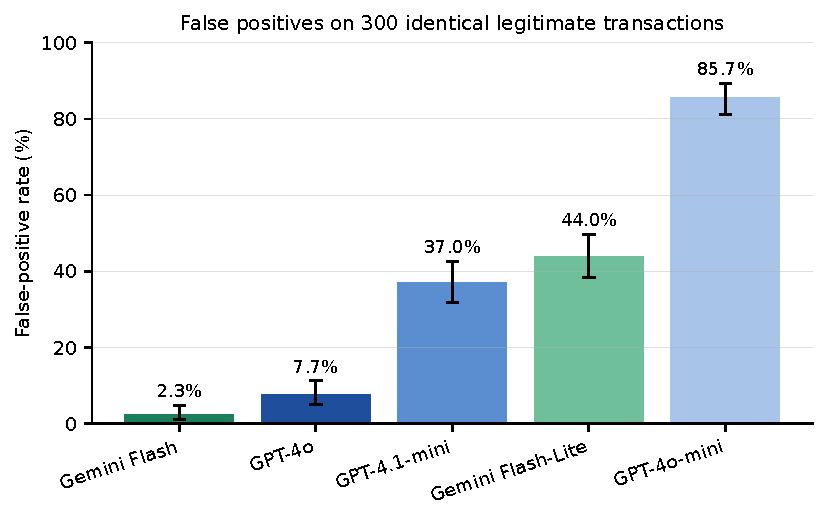
\includegraphics[width=0.72\textwidth]{fig1_fp_by_model.pdf}
\caption{\HLtag{Revised in revision}\textbf{False-positive rate of five foundation models on identical legitimate transactions.} Bars show the percentage of 300 legitimate cases each model flagged as suspicious. Error bars are 95\% Wilson score confidence intervals. Rates span 2.3--85.7\% (Cochran's $Q=585.0$, degrees of freedom $=4$, $P\approx2.7\times10^{-125}$)}
\label{fig:fp}
\end{figure}

\begin{figure}[t]
\centering
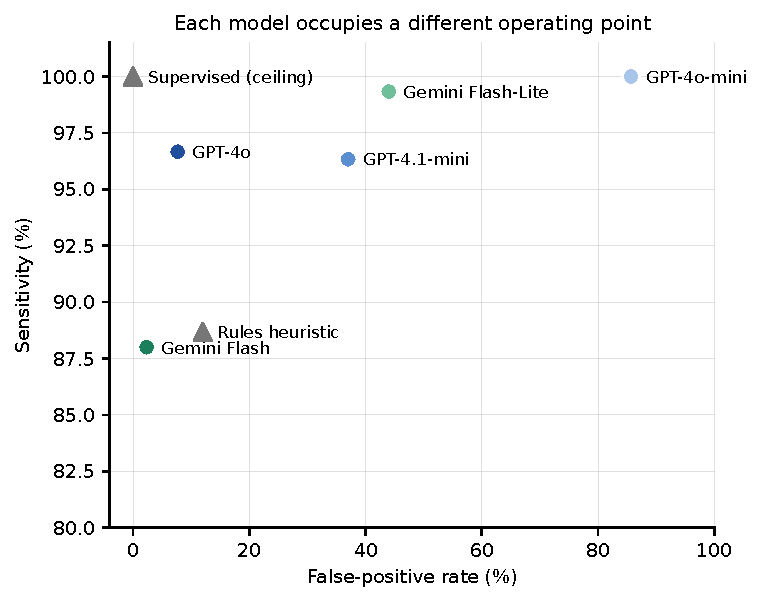
\includegraphics[width=0.62\textwidth]{fig2_operating_points.pdf}
\caption{\HLtag{Revised in revision}\textbf{Each model occupies a different operating point.} Sensitivity (percentage of 300 suspicious cases caught) versus false-positive rate (percentage of 300 legitimate cases flagged) for the five foundation models (circles) and the two non-LLM baselines (triangles: rules heuristic and supervised classifier). Within each provider in the evaluated model set, the more capable model is consistently associated with a lower false-positive rate}
\label{fig:ops}
\end{figure}

\begin{figure}[t]
\centering
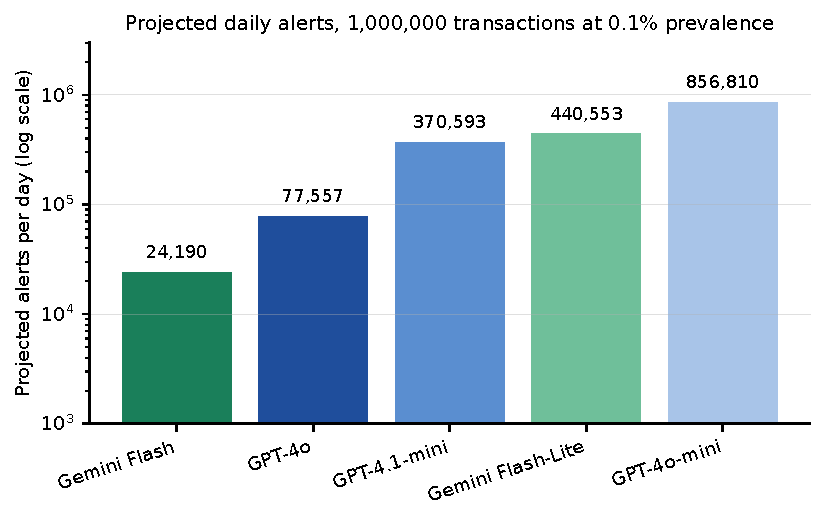
\includegraphics[width=0.72\textwidth]{fig3_alert_volume.pdf}
\caption{\HLtag{Revised in revision}\textbf{Projected daily alert workload under an illustrative low-prevalence scenario.} Expected daily alerts for each screener at a suspicious prevalence of 0.1\% over 1,000,000 transactions per day (logarithmic axis). Model choice changes the queue from about 24,000 to about 857,000 alerts on identical activity}
\label{fig:vol}
\end{figure}

\begin{figure}[t]
\centering
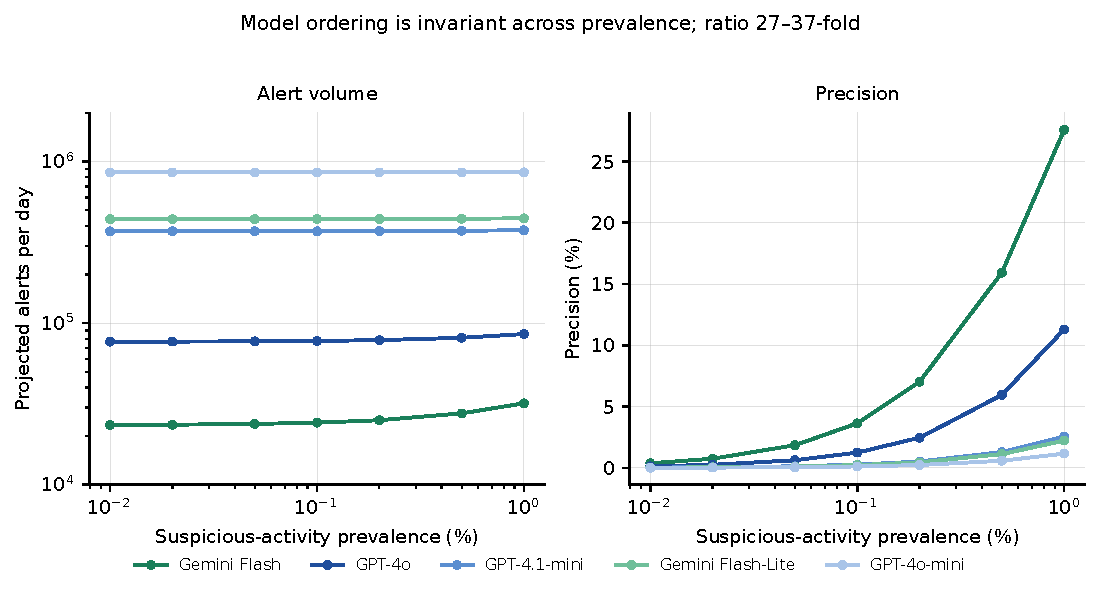
\includegraphics[width=0.95\textwidth]{fig6_prevalence_sweep.pdf}
\caption{\HLtag{New in revision}\textbf{Alert volume and precision across suspicious-activity prevalence.} Projected daily alerts (left) and precision (right) for each model over prevalence from 0.01\% to 1\%, at 1,000,000 transactions per day under the preregistered aggregation rule. The ordering of the five models is identical at every prevalence. The highest-to-lowest alert ratio moves from about 37-fold to about 27-fold across the swept range}
\label{fig:sweep}
\end{figure}

\begin{figure}[t]
\centering
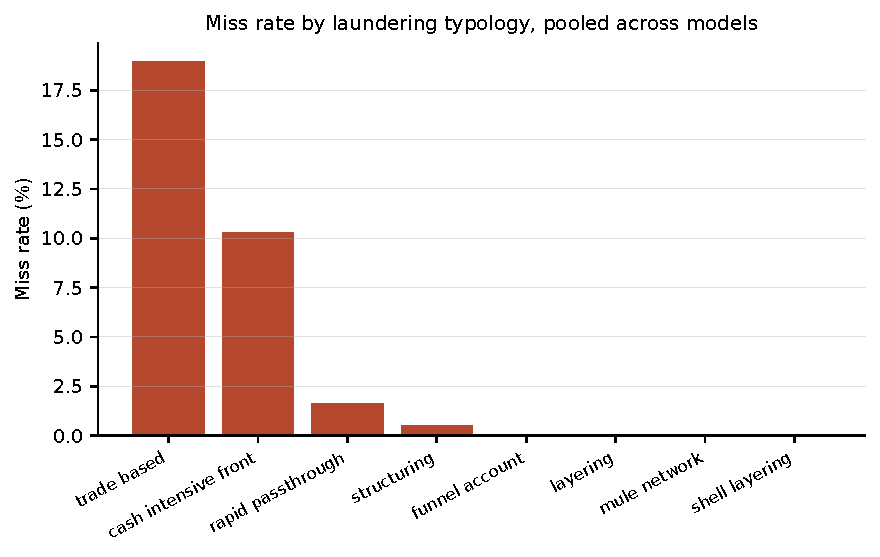
\includegraphics[width=0.75\textwidth]{fig4_typology_miss.pdf}
\caption{\HLtag{Revised in revision}\textbf{A shared blind spot for trade-based laundering.} Miss rate by laundering typology, pooled across the five models. Trade-based laundering and cash-intensive fronts are missed substantially more often than structural typologies}
\label{fig:typ}
\end{figure}

\begin{figure}[t]
\centering
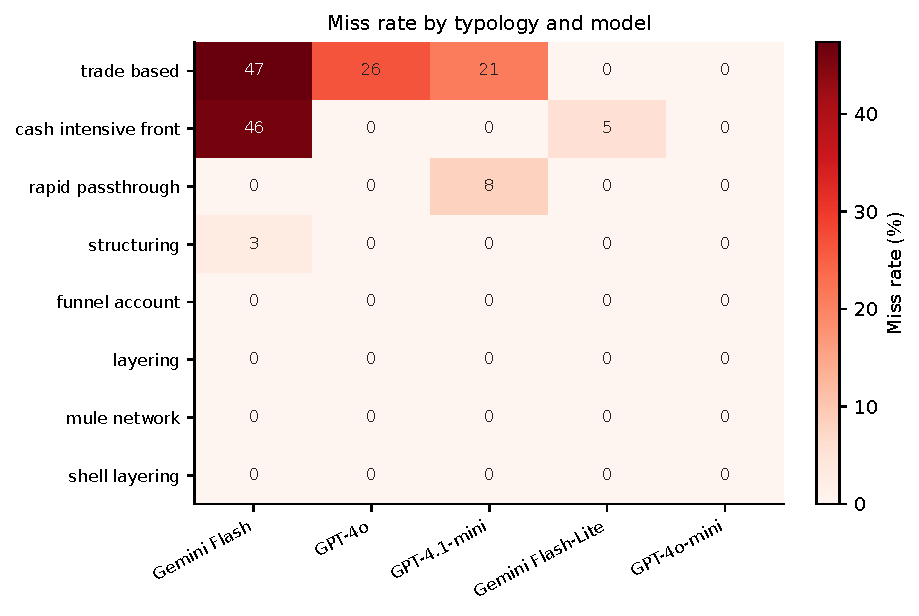
\includegraphics[width=0.66\textwidth]{fig5_typology_model_heatmap.pdf}
\caption{\HLtag{Revised in revision}\textbf{Miss rate by laundering typology and model.} Percentage of suspicious cases of each typology (rows) missed by each model (columns). Darker cells indicate more misses. The cautious models (Gemini Flash, GPT-4o) concentrate their misses in trade-based laundering and cash-intensive fronts, while the alert-flooding GPT-4o-mini misses almost nothing---the per-typology signature of the operating-point trade-off in Fig.~\ref{fig:ops}}
\label{fig:heat}
\end{figure}

\begin{table}[t]
\caption{\HLtag{Revised in revision}\textbf{Per-model operating point on the identical 600-case battery.} Values are percentages with 95\% Wilson score confidence intervals. Here $n=300$ legitimate and 300 suspicious cases.}\label{tab:ops}
\begin{tabular}{@{}llll@{}}
\toprule
Model & Provider & False-positive rate & Miss rate \\
\midrule
Gemini Flash      & Google & 2.3 [1.1--4.7] & 12.0 [8.8--16.2] \\
GPT-4o            & OpenAI & 7.7 [5.2--11.2] & 3.3 [1.8--6.0] \\
GPT-4.1-mini      & OpenAI & 37.0 [31.7--42.6] & 3.7 [2.1--6.4] \\
Gemini Flash-Lite & Google & 44.0 [38.5--49.7] & 0.7 [0.2--2.4] \\
GPT-4o-mini       & OpenAI & 85.7 [81.2--89.2] & 0.0 [0.0--1.3] \\
\botrule
\end{tabular}
\end{table}

\begin{table}[t]
\caption{\HLtag{Revised in revision}\textbf{Pairwise comparison of false-positive rates.} McNemar's exact (binomial) test on the 300 legitimate cases (same cases for all models). Here $b$ and $c$ are the discordant counts. $P$-values are two-tailed and Bonferroni-corrected across the ten model pairs. Pairs are ordered by corrected $P$. Nine of the ten comparisons are significant after correction. The single exception is GPT-4.1-mini versus Gemini Flash-Lite, two models occupying the same region of the operating-point space.}\label{tab:mcnemar}
\begin{tabular}{@{}lrrl@{}}
\toprule
Model pair & $b$ & $c$ & $P$ (Bonferroni) \\
\midrule
GPT-4.1-mini vs Gemini Flash-Lite      & 53 & 74 & 0.76 \\
Gemini Flash vs GPT-4o                 & 2 & 18 & $4.0\times10^{-3}$ \\
GPT-4o vs GPT-4.1-mini                 & 2 & 90 & $1.7\times10^{-23}$ \\
Gemini Flash-Lite vs GPT-4o-mini       & 12 & 137 & $4.9\times10^{-27}$ \\
GPT-4o vs Gemini Flash-Lite            & 4 & 113 & $9.2\times10^{-28}$ \\
Gemini Flash vs GPT-4.1-mini           & 2 & 106 & $3.6\times10^{-28}$ \\
Gemini Flash vs Gemini Flash-Lite      & 0 & 125 & $4.7\times10^{-37}$ \\
GPT-4.1-mini vs GPT-4o-mini            & 3 & 149 & $2.1\times10^{-39}$ \\
GPT-4o vs GPT-4o-mini                  & 0 & 234 & $7.2\times10^{-70}$ \\
Gemini Flash vs GPT-4o-mini            & 0 & 250 & $1.1\times10^{-74}$ \\
\botrule
\end{tabular}
\end{table}

\begin{table}[t]
\caption{\HLtag{Revised in revision}\textbf{Projected daily operational impact at 0.1\% prevalence (1,000,000 transactions/day).} Projected daily-alert counts show an FPR-uncertainty interval obtained by propagating the 95\% Wilson interval for the false-positive rate. Counts are rounded to three significant figures. Rules and supervised baselines are shown for reference. The supervised baseline is an optimistic ceiling on synthetic structure.}\label{tab:vol}
\begin{tabular}{@{}lrlr@{}}
\toprule
Screener & FP rate (\%) & Projected daily alerts (95\% CI) & Precision (\%) \\
\midrule
Supervised (ceiling) & 0.0  & $\sim$1{,}000                    & 100 \\
Gemini Flash         & 2.3 & 24{,}200 (12{,}200--48{,}200) & 3.6 \\
GPT-4o               & 7.7 & 77{,}600 (52{,}500--113{,}000) & 1.2 \\
Rules baseline       & 12.0 & 121{,}000 (88{,}700--162{,}000) & 0.7 \\
GPT-4.1-mini         & 37.0 & 371{,}000 (318{,}000--427{,}000) & 0.3 \\
Gemini Flash-Lite    & 44.0 & 441{,}000 (386{,}000--497{,}000) & 0.2 \\
GPT-4o-mini          & 85.7 & 857{,}000 (813{,}000--892{,}000) & 0.1 \\
\botrule
\end{tabular}
\end{table}

\begin{table}[t]
\caption{\HLtag{Revised in revision}\textbf{Per-case endpoint aggregation rule.} The rule was fixed in advance (preregistration decision~D4) and is label-independent: ties resolve toward \texttt{flag} on both legitimate and suspicious cases. It is applied identically to every model.}\label{tab:vote}
\begin{tabular}{@{}p{0.27\textwidth}p{0.63\textwidth}@{}}
\toprule
Element & Rule \\
\midrule
Replicate calls per case & The valid (non-ERROR) calls for each (model, case): four by design (two prompt phrasings $\times$ two seeds). 111 GPT-4o-mini cases carry a fifth retried call and one GPT-4.1-mini case carries three, which, with 9 ERROR rows, gives 12{,}120 realized calls against 12{,}000 by design. All valid calls, including the 111 duplicates, enter the vote (Section~\ref{sec:design}) \\
Failed / unparsable calls & Recorded as ERROR and excluded from the vote (the denominator is reduced accordingly). Overall ERROR rate 0.08\% \\
Legitimate (benign) case & Counted as a false positive if at least half of the valid calls flagged it (flags $\geq$ half). A 2--2 tie is counted as a false positive \\
Suspicious case & Counted as caught (not missed) if at least half of the valid calls flagged it (flags $\geq$ half). A 2--2 tie is counted as caught \\
Even-split ties & Resolved toward \texttt{flag} on both labels, affecting 132 of the 1{,}500 legitimate and 48 of the 1{,}500 suspicious model--case decisions. Per model the legitimate-case counts are 6, 20, 40, 58 and 8 for Gemini Flash, GPT-4o, GPT-4.1-mini, Gemini Flash-Lite and GPT-4o-mini, and the suspicious-case counts 19, 15, 10, 4 and 0 \\
Deviation at submission & The submitted analysis required a strict majority on legitimate cases, making the tie direction depend on the case label. Corrected here. See Section~\ref{sec:agg} \\
\botrule
\end{tabular}
\end{table}

\clearpage
\backmatter

\bmhead{Acknowledgements}
Analyses used open-source software (Python, NumPy, scikit-learn, SciPy, \HLdel{Matplotlib); the} \HLtext{Matplotlib). The} authors thank the maintainers of these open-source projects.

\section*{Declarations}

\textbf{Funding.} No funding was received for this study.

\textbf{Author contributions.} S.C. conceived the study, designed and preregistered the analysis, implemented the data-collection and analysis software, performed the experiments and analysis, and produced the figures. R.C. contributed to the study design, the interpretation of results, and the critical revision of the manuscript. Both authors wrote, reviewed and approved the final manuscript.

\textbf{Data availability.} All data and code required to reproduce the study are openly available in the public GitHub repository at \url{https://github.com/samirrc2/ai-foundation-model-aml-false-positives} \HLdel{(MIT licence); the} \HLtext{under the MIT licence, and archived on Zenodo under the concept DOI} \url{https://doi.org/10.5281/zenodo.23424852}\HLtext{, which resolves to the most recent version. The} repository root includes \texttt{REPRODUCIBILITY\_DOCUMENTATION.pdf}, a \HLdel{section-by-section guide to every input, script,} \HLtext{guide to every input, script} and output and to the \HLtext{offline reproduction, which runs with one command.} The study uses only synthetic \HLdel{data: no human participants, no proprietary records, and no live model access are needed} \HLtext{transaction data. No human participants, proprietary records or live model access are required} to reproduce any result.

\textbf{Code availability.} The analysis and reproducibility code---which regenerates and hash-verifies the battery, recomputes every reported statistic, and confirms byte-identical outputs across runs---is available in the same GitHub repository (\url{https://github.com/samirrc2/ai-foundation-model-aml-false-positives}\HLdel{); its} \HLtext{). Its} use is documented in \texttt{REPRODUCIBILITY\_DOCUMENTATION.pdf} at the repository root. The default offline reproduction requires no API keys or network access. The code is released under the MIT licence.

\textbf{Competing interests.} The authors declare no competing interests.

\textbf{Ethics approval and consent to participate.} Not \HLdel{applicable (synthetic data only;} \HLtext{applicable. The study uses synthetic data only, with} no human participants, human tissue or \HLdel{animals).} \HLdel{\textbf{Consent for publication.} Not applicable.} \HLdel{\textbf{Materials availability.} Not applicable (the} \HLtext{animals.}

\textbf{Consent for publication.} \HLtext{Not applicable.}

\textbf{Materials availability.} \HLtext{Not applicable. The} study uses only synthetic data and open-source \HLdel{software; no physical materials).} \HLtext{software, with no physical materials.}

\textbf{Generative AI use.} Generative AI (Anthropic Claude) was used to assist with software scaffolding, development and coding of the analysis and reproducibility pipeline, and with grammar correction and minor language edits of the authors' own text, in all cases under the authors' direction. Separately, five commercially available large language models are the object of study and the measurement instrument of this work---their automated transaction screening is exactly what is being evaluated---as described in Methods. No large language model is listed as an author. The authors reviewed and verified all such output and take full responsibility for the content, consistent with the journal's authorship policy.

\textbf{ORCID.} S.C. \HLdel{0009-0007-2779-3492;} \HLtext{0009-0007-2779-3492,} R.C. 0009-0007-2807-3948.

\bibliography{references_discover}

\end{document}
